\chapter{Simulation Model Development}

\addcontentsline{toc}{chapter}{Simulation Model Development}

\section{Main Entities}

This chapter is going to describe the process of implementation, i.e. transition from a mathematical model to computer simulation.

\begin{figure}
    \centering
    \begin{subfigure}[b]{0.3\textwidth}
        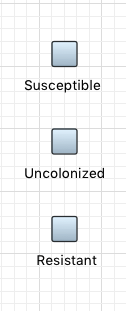
\includegraphics[width=\textwidth]{img/screens/basic/basic4}
        \caption{A gull}
        \label{fig:gull}
    \end{subfigure}
    ~ %add desired spacing between images, e. g. ~, \quad, \qquad, \hfill etc.
      %(or a blank line to force the subfigure onto a new line)
    \begin{subfigure}[b]{0.3\textwidth}
        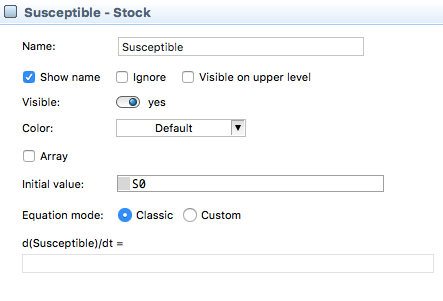
\includegraphics[width=\textwidth]{img/screens/basic/basic3}
        \caption{A tiger}
        \label{fig:tiger}
    \end{subfigure}
\end{figure}